\documentclass[11pt,a4paper]{report}
\usepackage[textwidth=37em,vmargin=30mm]{geometry}
\usepackage{calc,xunicode,amsmath,amssymb,paralist,enumitem,tabu,booktabs,datetime2,xeCJK,xeCJKfntef,listings}
\usepackage{tocloft,fancyhdr,tcolorbox,xcolor,graphicx,eso-pic,xltxtra,xelatexemoji}

\newcommand{\envyear}[0]{2025}
\newcommand{\envdatestr}[0]{2025-03-26}
\newcommand{\envfinaldir}[0]{webdb/2025/20250326/final}

\usepackage[hidelinks]{hyperref}
\hypersetup{
    colorlinks=false,
    pdfpagemode=FullScreen,
    pdftitle={Web Digest - \envdatestr}
}

\setlength{\cftbeforechapskip}{10pt}
\renewcommand{\cftchapfont}{\rmfamily\bfseries\large\raggedright}
\setlength{\cftbeforesecskip}{2pt}
\renewcommand{\cftsecfont}{\sffamily\small\raggedright}

\setdefaultleftmargin{2em}{2em}{1em}{1em}{1em}{1em}

\usepackage{xeCJK,xeCJKfntef}
\xeCJKsetup{PunctStyle=plain,RubberPunctSkip=false,CJKglue=\strut\hskip 0pt plus 0.1em minus 0.05em,CJKecglue=\strut\hskip 0.22em plus 0.2em}
\XeTeXlinebreaklocale "zh"
\XeTeXlinebreakskip = 0pt


\setmainfont{Brygada 1918}
\setromanfont{Brygada 1918}
\setsansfont{IBM Plex Sans}
\setmonofont{JetBrains Mono NL}
\setCJKmainfont{Noto Serif CJK SC}
\setCJKromanfont{Noto Serif CJK SC}
\setCJKsansfont{Noto Sans CJK SC}
\setCJKmonofont{Noto Sans CJK SC}

\setlength{\parindent}{0pt}
\setlength{\parskip}{8pt}
\linespread{1.15}

\lstset{
	basicstyle=\ttfamily\footnotesize,
	numbersep=5pt,
	backgroundcolor=\color{black!5},
	showspaces=false,
	showstringspaces=false,
	showtabs=false,
	tabsize=2,
	captionpos=b,
	breaklines=true,
	breakatwhitespace=true,
	breakautoindent=true,
	linewidth=\textwidth
}






\newcommand{\coverpic}[2]{
    % argv: itemurl, authorname
    Cover photo by #2~~(\href{#1}{#1})
}
\newcommand{\makeheader}[0]{
    \begin{titlepage}
        % \newgeometry{hmargin=15mm,tmargin=21mm,bmargin=12mm}
        \begin{center}
            
            \rmfamily\scshape
            \fontspec{BaskervilleF}
            \fontspec{Old Standard}
            \fontsize{59pt}{70pt}\selectfont
            WEB\hfill DIGEST
            
            \vfill
            % \vskip 30pt
            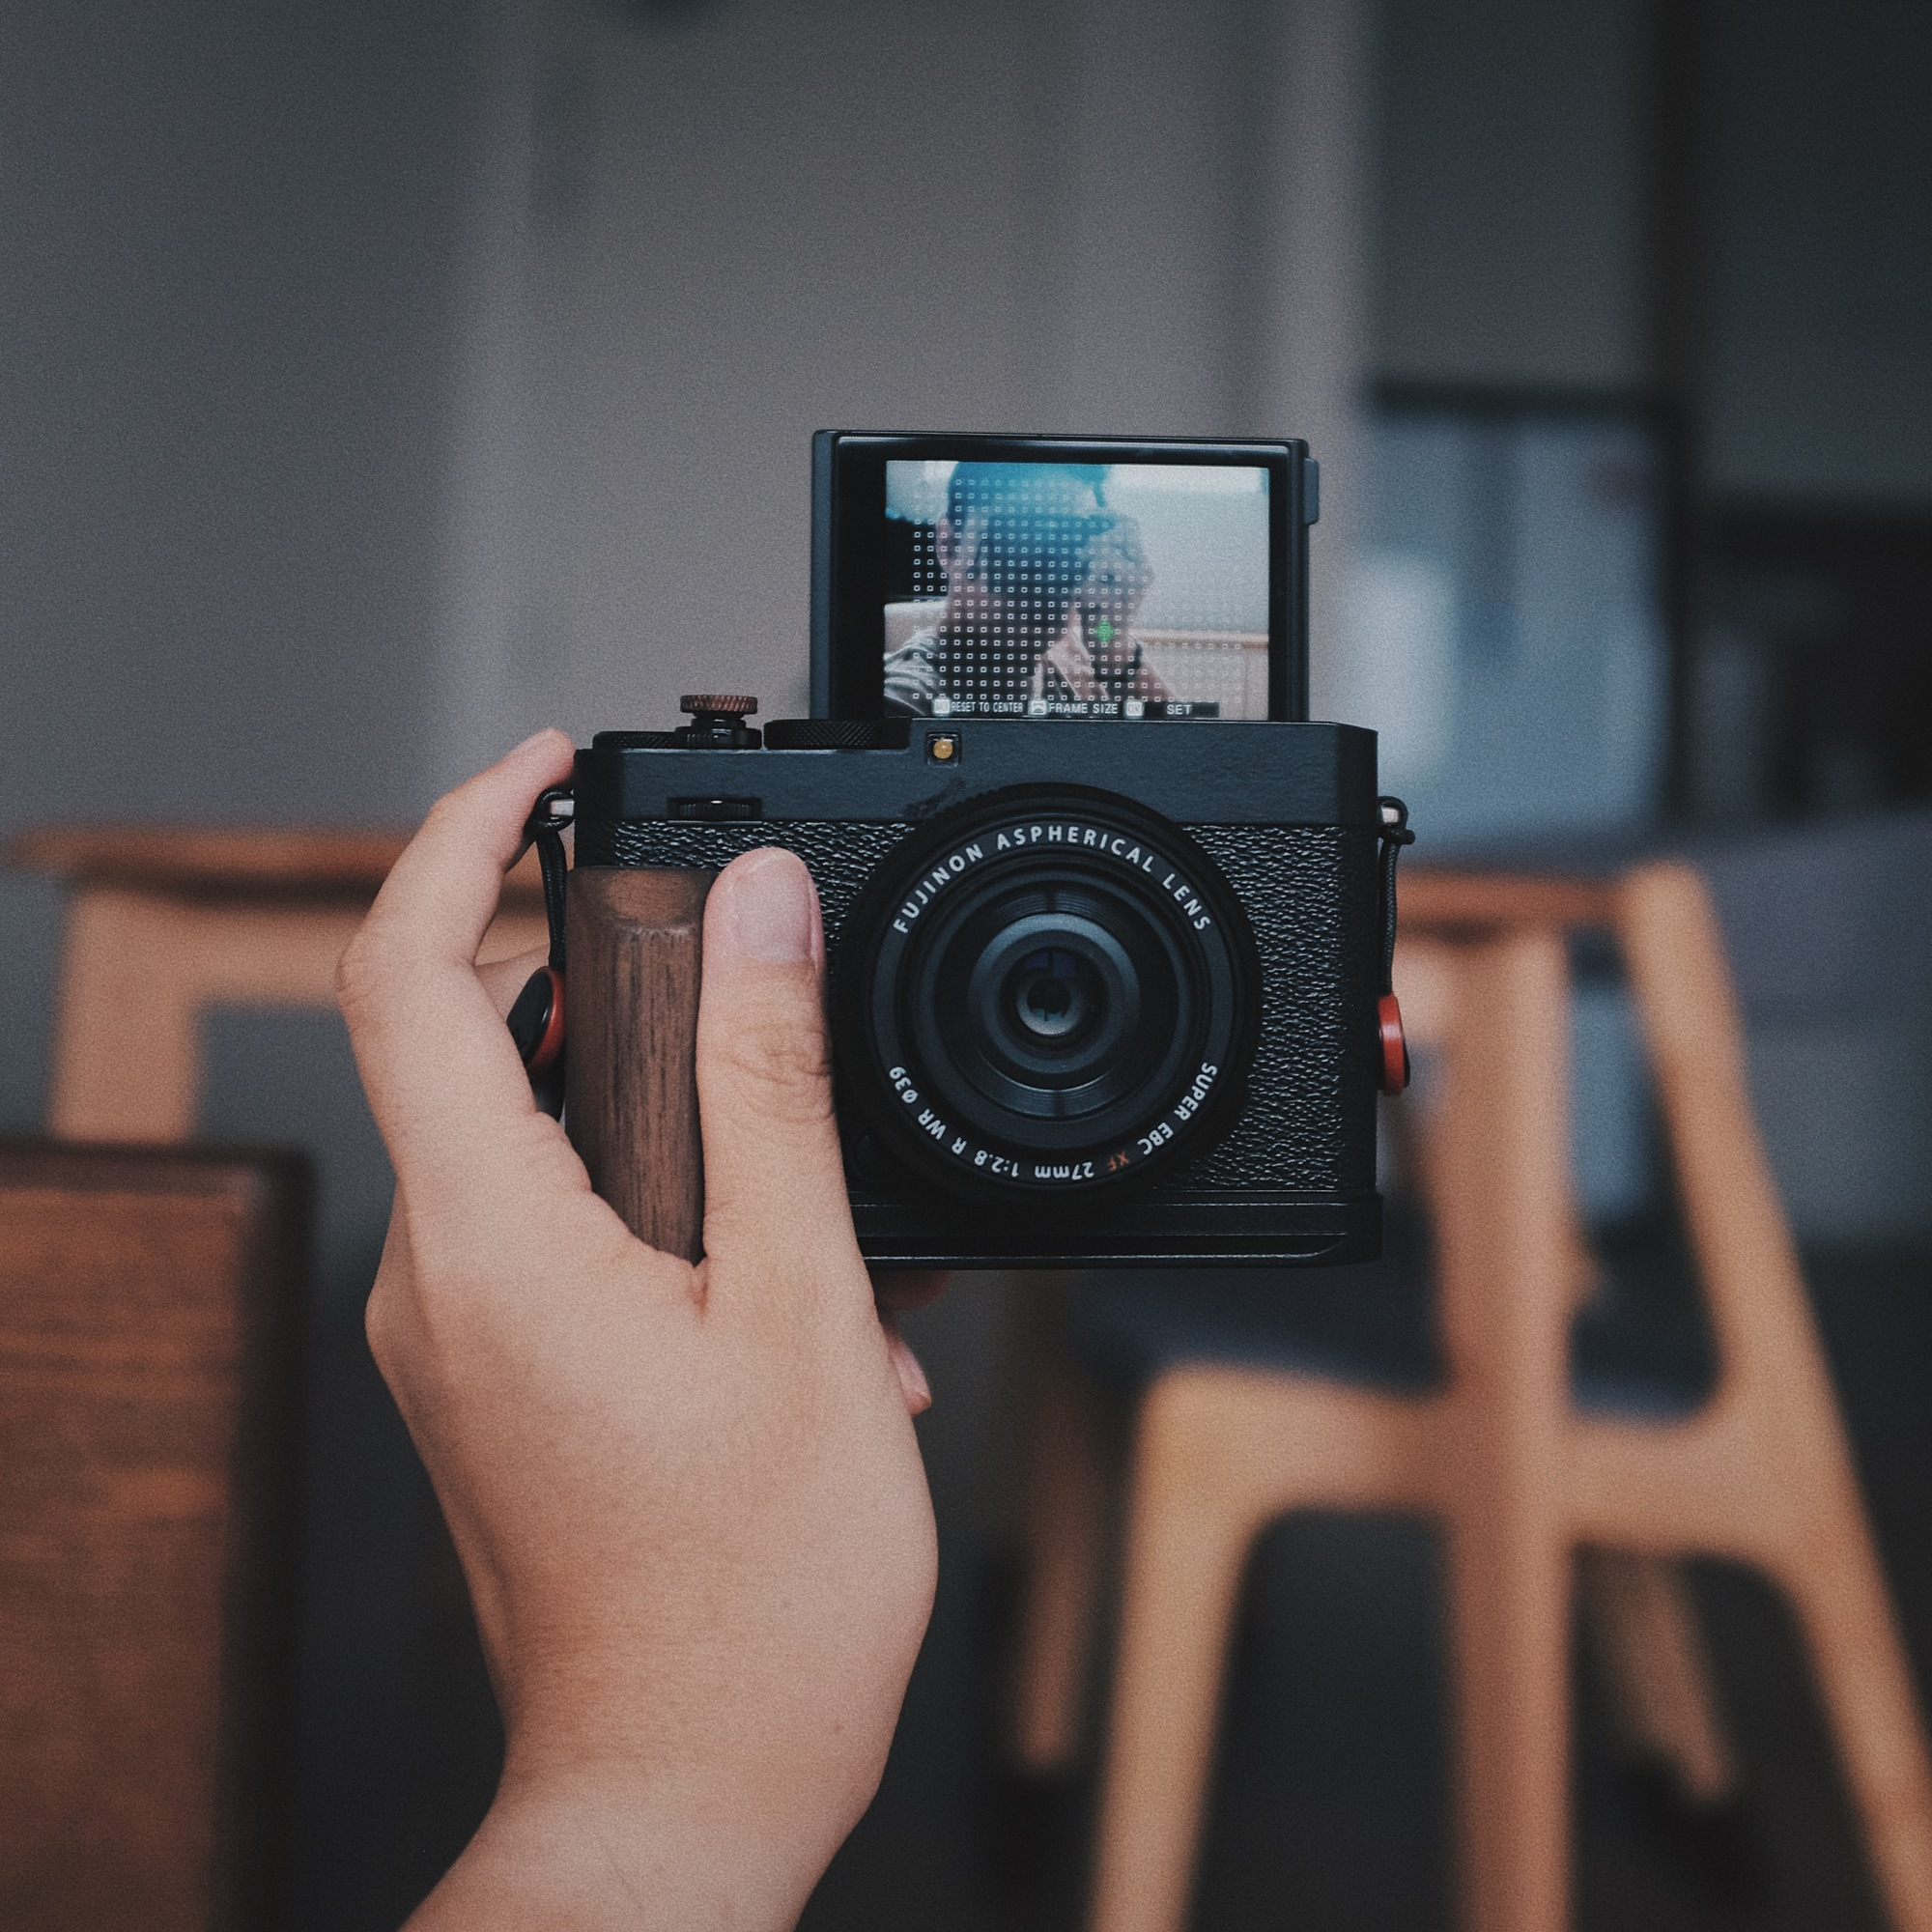
\includegraphics[width=\linewidth]{\envfinaldir/coverpic-prod.jpg}\par
            % \vskip 30pt
            \vfill

            \normalsize\rmfamily\scshape
            \copyright{} The Web Digest Project \hfill\large \envdatestr
        \end{center}
    \end{titlepage}
    % \restoregeometry
}
\newcommand{\simplehref}[1]{%
    \textcolor{blue!80!green}{\href{#1}{#1}}%
}
\renewcommand{\contentsname}{\center\Huge\sffamily\bfseries Contents\par\vskip 20pt}
\newcounter{ipartcounter}
\setcounter{ipartcounter}{0}
\newcommand{\ipart}[1]{
    % \vskip 20pt
    \clearpage
    \stepcounter{ipartcounter}
    \phantomsection
    \addcontentsline{toc}{chapter}{#1}
    % \begin{center}
    %     \Huge
    %     \sffamily\bfseries
    %     #1
    % \end{center}
    % \vskip 20pt plus 7pt
}
\newcounter{ichaptercounter}
\setcounter{ichaptercounter}{0}
\newcommand{\ichapter}[1]{
    % \vskip 20pt
    \clearpage
    \stepcounter{ichaptercounter}
    \phantomsection
    \addcontentsline{toc}{section}{\numberline{\arabic{ichaptercounter}}#1}
    \begin{center}
        \Huge
        \sffamily\bfseries
        #1
    \end{center}
    \vskip 20pt plus 7pt
}
\newcommand{\entrytitlefont}[1]{\subsection*{\raggedright\Large\sffamily\bfseries#1}}
\newcommand{\entryitemGeneric}[2]{
    % argv: title, url
    \parbox{\linewidth}{
        \entrytitlefont{#1}\par\vskip 5pt
        \footnotesize\ttfamily\mdseries
        \simplehref{#2}
    }\vskip 11pt plus 11pt minus 1pt
}
\newcommand{\entryitemGithub}[3]{
    % argv: title, url, desc
    \parbox{\linewidth}{
        \entrytitlefont{#1}\par\vskip 5pt
        \footnotesize\ttfamily\mdseries
        \simplehref{#2}\par\vskip 5pt
        \small\rmfamily\mdseries#3
    }\vskip 11pt plus 11pt minus 1pt
}
\newcommand{\entryitemAp}[3]{
    % argv: title, url, desc
    \parbox{\linewidth}{
        \entrytitlefont{#1}\par\vskip 5pt
        \footnotesize\ttfamily\mdseries
        \simplehref{#2}\par\vskip 5pt
        \small\rmfamily\mdseries#3
    }\vskip 11pt plus 11pt minus 1pt
}
\newcommand{\entryitemHackernews}[3]{
    % argv: title, hnurl, rawurl
    % \parbox{\linewidth}{
    %     \entrytitlefont{#1}\par\vskip 5pt
    %     \footnotesize\ttfamily\mdseries
    %     \simplehref{#3}\par
    %     \textcolor{black!50}{\href{#2}{#2}}
    % }\vskip 11pt plus 11pt minus 1pt
    \begin{minipage}{\linewidth}
            \entrytitlefont{#1}\par\vskip 5pt
            \footnotesize\ttfamily\mdseries
            \simplehref{#3}\par
            \textcolor{black!50}{\href{#2}{#2}}
    \end{minipage}\par\vskip 11pt plus 11pt minus 1pt
}







\begin{document}

\makeheader

\tableofcontents\clearpage




\ipart{Developers}
\ichapter{Hacker News}
\entryitemTwoLinks{In Jail Without a Lawyer: How a Texas Town Fails Poor Defendants}{https://news.ycombinator.com/item?id=43474593}{https://www.nytimes.com/2025/03/25/us/maverick-county-texas-court-system.html}

\entryitemTwoLinks{The highest-ranking personal blogs of Hacker News}{https://news.ycombinator.com/item?id=43474505}{https://refactoringenglish.com/tools/hn-popularity/}

\entryitemTwoLinks{4o Image Generation}{https://news.ycombinator.com/item?id=43474112}{https://openai.com/index/introducing-4o-image-generation/}

\entryitemTwoLinks{Stoop Coffee: A simple idea transformed my neighborhood}{https://news.ycombinator.com/item?id=43473618}{https://supernuclear.substack.com/p/stoop-coffee-how-a-simple-idea-transformed}

\entryitemTwoLinks{Gemini 2.5}{https://news.ycombinator.com/item?id=43473489}{https://blog.google/technology/google-deepmind/gemini-model-thinking-updates-march-2025/}

\entryitemTwoLinks{Kylie Minogue song about a typeface}{https://news.ycombinator.com/item?id=43473358}{https://abcdinamo.com/news/german-bold-italic}

\entryitemTwoLinks{Why is C the symbol for the speed of light? (2004)}{https://news.ycombinator.com/item?id=43472663}{https://math.ucr.edu/home/baez/physics/Relativity/SpeedOfLight/c.html}

\entryitemTwoLinks{If you get the chance, always run more extra network fiber cabling}{https://news.ycombinator.com/item?id=43471177}{https://utcc.utoronto.ca/~cks/space/blog/sysadmin/RunMoreExtraNetworkFiber}

\entryitemTwoLinks{Open-sourcing OpenPubkey SSH (OPKSSH): integrating single sign-on with SSH}{https://news.ycombinator.com/item?id=43470906}{https://blog.cloudflare.com/open-sourcing-openpubkey-ssh-opkssh-integrating-single-sign-on-with-ssh/}

\entryitemTwoLinks{An AI bubble threatens Silicon Valley, and all of us}{https://news.ycombinator.com/item?id=43470786}{https://prospect.org/power/2025-03-25-bubble-trouble-ai-threat/}

\entryitemTwoLinks{Tesla deliveries down 43\% in Europe while EVs are up 31\%}{https://news.ycombinator.com/item?id=43470763}{https://electrek.co/2025/03/25/tesla-tsla-deliveries-down-43-in-europe-while-evs-are-up-28/}

\entryitemTwoLinks{Samsung CEO Jong-hee Han has died}{https://news.ycombinator.com/item?id=43470699}{https://www.engadget.com/big-tech/samsung-ceo-jong-hee-han-has-died-120029286.html}

\entryitemTwoLinks{VGGT: Visual Geometry Grounded Transformer}{https://news.ycombinator.com/item?id=43470651}{https://github.com/facebookresearch/vggt}

\entryitemTwoLinks{X's director of engineering, Haofei Wang, has left the company}{https://news.ycombinator.com/item?id=43470613}{https://www.theverge.com/twitter/634833/x-head-engineering-leaves-elon-musk}

\entryitemTwoLinks{Coding Isn't Programming}{https://news.ycombinator.com/item?id=43469711}{https://www.socallinuxexpo.org/scale/22x/presentations/closing-keynote-leslie-lamport}

\entryitemTwoLinks{The Great Barefoot Running Hysteria of 2010}{https://news.ycombinator.com/item?id=43469690}{https://runningshoescore.com/blog/barefoot-running-hysteria-of-2010}

\entryitemTwoLinks{Spammers are better at SPF, DKIM, and DMARC than everyone else}{https://news.ycombinator.com/item?id=43468995}{https://toad.social/@grumpybozo/114213600922816869}

\entryitemTwoLinks{Writing your own C++ standard library from scratch}{https://news.ycombinator.com/item?id=43468976}{https://nibblestew.blogspot.com/2025/03/writing-your-own-c-standard-library.html}

\entryitemTwoLinks{A Sneaky Phish Just Grabbed My Mailchimp Mailing List}{https://news.ycombinator.com/item?id=43468959}{https://www.troyhunt.com/a-sneaky-phish-just-grabbed-my-mailchimp-mailing-list/}

\entryitemTwoLinks{Reflecting on WikiTok}{https://news.ycombinator.com/item?id=43468491}{https://www.aizk.sh/posts/reflecting-on-wikitok}\ichapter{Phoronix}
\entryitemGeneric{\hskip 0pt{}XZ 5.8 Debuts As First Major Feature Release Since The Backdoor Disaster}{https://www.phoronix.com/news/XZ-5.8-Released}

\entryitemGeneric{\hskip 0pt{}MPV 0.40 Media Player Released With Wayland HDR Support}{https://www.phoronix.com/news/MPV-0.40-Released}

\entryitemGeneric{\hskip 0pt{}NVIDIA GeForce RTX 5070 Linux Gaming/Graphics Performance}{https://www.phoronix.com/review/nvidia-rtx5070-linux-gaming}

\entryitemGeneric{\hskip 0pt{}Fwupd 2.0.7 Released With New Plug-Ins \& Additional Hardware Support}{https://www.phoronix.com/news/Fwupd-2.0.7-Released}

\entryitemGeneric{\hskip 0pt{}Latest Batch Of Rust Compiler Updates For GCC 15.1 Lands Support For... For Loops}{https://www.phoronix.com/news/Gccrs-Rust-GCC-15-For-Loops}

\entryitemGeneric{\hskip 0pt{}Intel Engineer Posts Cache-Aware Load Balancing For Linux - May Be Very Useful For AMD}{https://www.phoronix.com/news/Linux-Cache-Aware-Load-Balance}

\entryitemGeneric{\hskip 0pt{}F2FS Sees Nice Set Of Enhancements For Linux 6.15}{https://www.phoronix.com/news/F2FS-Linux-6.15}

\entryitemGeneric{\hskip 0pt{}GCC \& LLVM Clang Merge Support For The NVIDIA Olympus Cores With The Vera CPU}{https://www.phoronix.com/news/NVIDIA-Olympus-GCC-Clang}

\entryitemGeneric{\hskip 0pt{}AMD INVLPGB Merged For Linux 6.15 To Provide Another Performance Advantage}{https://www.phoronix.com/news/AMD-INVLPGB-Merged-Linux-6.15}\ichapter{Dribbble}
\entryitemGeneric{\hskip 0pt{}Crypto Portfolio Tracker App}{https://dribbble.com/shots/25820014-Crypto-Portfolio-Tracker-App}

\entryitemGeneric{\hskip 0pt{}Aura - Logo Design}{https://dribbble.com/shots/25815819-Aura-Logo-Design}

\entryitemGeneric{\hskip 0pt{}Complexure}{https://dribbble.com/shots/25815646-Complexure}

\entryitemGeneric{\hskip 0pt{}Snitcher - New Branding}{https://dribbble.com/shots/25816140-Snitcher-New-Branding}

\entryitemGeneric{\hskip 0pt{}Spark illustrations}{https://dribbble.com/shots/25815705-Spark-illustrations}

\entryitemGeneric{\hskip 0pt{}Lepisov Branding Logo Reveal Animation}{https://dribbble.com/shots/25814536-Lepisov-Branding-Logo-Reveal-Animation}

\entryitemGeneric{\hskip 0pt{}FCKD}{https://dribbble.com/shots/25812257-FCKD}

\entryitemGeneric{\hskip 0pt{}Task completion micro interaction}{https://dribbble.com/shots/25797132-Task-completion-micro-interaction}

\entryitemGeneric{\hskip 0pt{}Phantom auto buy/sell concept}{https://dribbble.com/shots/25799751-Phantom-auto-buy-sell-concept}

\entryitemGeneric{\hskip 0pt{}Crypto App Design}{https://dribbble.com/shots/25801686-Crypto-App-Design}

\entryitemGeneric{\hskip 0pt{}PurePaws - Logo Design}{https://dribbble.com/shots/25797575-PurePaws-Logo-Design}

\entryitemGeneric{\hskip 0pt{}S mark}{https://dribbble.com/shots/25796446-S-mark}

\entryitemGeneric{\hskip 0pt{}Central Coast}{https://dribbble.com/shots/25794367-Central-Coast}

\entryitemGeneric{\hskip 0pt{}The Sequencer Poster}{https://dribbble.com/shots/25798231-The-Sequencer-Poster}

\entryitemGeneric{\hskip 0pt{}PieLabs Unused Character}{https://dribbble.com/shots/25797256-PieLabs-Unused-Character}

\entryitemGeneric{\hskip 0pt{}Puzzle Fintech UI/UX design, User Interface experience}{https://dribbble.com/shots/25652036-Puzzle-Fintech-UI-UX-design-User-Interface-experience}

\entryitemGeneric{\hskip 0pt{}Novascan}{https://dribbble.com/shots/25790443-Novascan}

\entryitemGeneric{\hskip 0pt{}Decades of Unforgettable Hits}{https://dribbble.com/shots/25792477-Decades-of-Unforgettable-Hits}

\entryitemGeneric{\hskip 0pt{}Plain - Branding}{https://dribbble.com/shots/25790107-Plain-Branding}

\entryitemGeneric{\hskip 0pt{}Mixed Stickers}{https://dribbble.com/shots/25737407-Mixed-Stickers}

\entryitemGeneric{\hskip 0pt{}Halo Movie poster}{https://dribbble.com/shots/25791667-Halo-Movie-poster}

\entryitemGeneric{\hskip 0pt{}Finory app}{https://dribbble.com/shots/25778453-Finory-app}

\entryitemGeneric{\hskip 0pt{}Lemur}{https://dribbble.com/shots/25792165-Lemur}

\entryitemGeneric{\hskip 0pt{}Delivery Mobile App Design}{https://dribbble.com/shots/25743029-Delivery-Mobile-App-Design}


\ipart{Developers~~~~(zh-Hans)}
\ichapter{Solidot}
\entryitemGeneric{\hskip 0pt{}李开复称中美 AI 差距仅为三个月}{https://www.solidot.org/story?sid=80881}

\entryitemGeneric{\hskip 0pt{}科学家寻求更精确的测量疼痛}{https://www.solidot.org/story?sid=80880}

\entryitemGeneric{\hskip 0pt{}银河系中心的龙卷风}{https://www.solidot.org/story?sid=80879}

\entryitemGeneric{\hskip 0pt{}如何减少 AI 大模型的功耗}{https://www.solidot.org/story?sid=80878}

\entryitemGeneric{\hskip 0pt{}2024 年全球气候多项指标创下记录}{https://www.solidot.org/story?sid=80877}

\entryitemGeneric{\hskip 0pt{}家族企业表现出更多环境责任行为}{https://www.solidot.org/story?sid=80876}

\entryitemGeneric{\hskip 0pt{}最新观测挑战宇宙标准模型}{https://www.solidot.org/story?sid=80875}

\entryitemGeneric{\hskip 0pt{}Google 和计算机历史博物馆发布 AlexNet 源代码}{https://www.solidot.org/story?sid=80874}

\entryitemGeneric{\hskip 0pt{}中国依靠工程师红利挑战美国的科技主导地位}{https://www.solidot.org/story?sid=80873}

\entryitemGeneric{\hskip 0pt{}FaunaDB 倒闭,计划开源}{https://www.solidot.org/story?sid=80872}

\entryitemGeneric{\hskip 0pt{}大西洋月刊主编被拉入一个讨论轰炸也门计划的 Signal 群聊中}{https://www.solidot.org/story?sid=80871}

\entryitemGeneric{\hskip 0pt{}库克访华,宣布设立 7.2 亿元清洁能源投资基金}{https://www.solidot.org/story?sid=80870}

\entryitemGeneric{\hskip 0pt{}Linux Kernel 6.14 释出}{https://www.solidot.org/story?sid=80869}

\entryitemGeneric{\hskip 0pt{}波音将为美国空军制造下一代隐形战斗机 F-47}{https://www.solidot.org/story?sid=80868}

\entryitemGeneric{\hskip 0pt{}European Alternatives 网站今年至今吸引了逾百万访客}{https://www.solidot.org/story?sid=80866}

\entryitemGeneric{\hskip 0pt{}Facebook 告密者寻求推翻采访禁令}{https://www.solidot.org/story?sid=80865}

\entryitemGeneric{\hskip 0pt{}已知最遥远星系中发现氧元素}{https://www.solidot.org/story?sid=80864}

\entryitemGeneric{\hskip 0pt{}23andMe 申请破产保护}{https://www.solidot.org/story?sid=80863}

\entryitemGeneric{\hskip 0pt{}AI 编程助手能通过规则文件生成后门}{https://www.solidot.org/story?sid=80862}

\entryitemGeneric{\hskip 0pt{}摧毁x86最后堡垒:Intel电熔丝e-Fuse加密密钥泄漏}{https://www.solidot.org/story?sid=80861}\ichapter{V2EX}
\entryitemGeneric{\hskip 0pt{}[macOS] MacBook pro 无故锁屏熄屏}{https://www.v2ex.com/t/1121074}

\entryitemGeneric{\hskip 0pt{}[Apple] ios 为什么不能统计副卡的流量总和}{https://www.v2ex.com/t/1121073}

\entryitemGeneric{\hskip 0pt{}[分享创造] 做了一个 HackerNews 榜单🔥,自带 AI 翻译、AI 总结、文章封面,支持 RSS}{https://www.v2ex.com/t/1121072}

\entryitemGeneric{\hskip 0pt{}[职场话题] 大四留级一年时间,从 Java 换行请问有推荐的赛道吗}{https://www.v2ex.com/t/1121071}

\entryitemGeneric{\hskip 0pt{}[北京] 深夜 1 点多,被人拽了一下床}{https://www.v2ex.com/t/1121070}

\entryitemGeneric{\hskip 0pt{}[NAS] 6 路监控摄像头 存储到 nas 有什么好的方案吗?}{https://www.v2ex.com/t/1121069}

\entryitemGeneric{\hskip 0pt{}[推广] 德国 ESIM 卡 8.99 欧每个月 15G 和无限通话时间+短信,用优惠码可以白嫖前两月}{https://www.v2ex.com/t/1121068}

\entryitemGeneric{\hskip 0pt{}[问与答] 畅网 N100 软路由死机频繁, PVE + 爱快 + IstoreOS 配置,换硬盘后仍未解决,求助!}{https://www.v2ex.com/t/1121067}

\entryitemGeneric{\hskip 0pt{}[VXNA] 申请收录博客:随机森林}{https://www.v2ex.com/t/1121066}

\entryitemGeneric{\hskip 0pt{}[.NET] 项目从.NET5.0 升级到 8.0,加起来 1.5 万行代码, Linux 下编译经常要半个小时,有的时候又几秒钟就能编译完, Windows 下一直非常正常,怎么排查?}{https://www.v2ex.com/t/1121065}

\entryitemGeneric{\hskip 0pt{}[健康] 有拔过阻生齿智齿的朋友没,有没有什么注意事项。}{https://www.v2ex.com/t/1121063}

\entryitemGeneric{\hskip 0pt{}[随想] 出了个乌龙,被各个 AI 搞的恍惚了。}{https://www.v2ex.com/t/1121062}

\entryitemGeneric{\hskip 0pt{}[Apple] Plex 现在 278 即可开通 Lifetime}{https://www.v2ex.com/t/1121061}

\entryitemGeneric{\hskip 0pt{}[程序员] 请教,专线和家庭宽带到底有哪些区别?一个 200 人的公司只用家庭宽带可不可行?}{https://www.v2ex.com/t/1121059}

\entryitemGeneric{\hskip 0pt{}[OpenWrt] 为什么使用 openwrt+bypass,有的网站必须清理我本地 dns 才能打开}{https://www.v2ex.com/t/1121057}

\entryitemGeneric{\hskip 0pt{}[酷工作] [长沙] 蚂蚁国际-数字马力招聘应用安全工程师}{https://www.v2ex.com/t/1121056}

\entryitemGeneric{\hskip 0pt{}[程序员] 听说 Deepseek v3 编程能力大幅提高 有什么能调用 V3 并且国内免翻的类 cursor 工具呢}{https://www.v2ex.com/t/1121055}

\entryitemGeneric{\hskip 0pt{}[iOS] 快讯: loon 内测版本支持 reality 了}{https://www.v2ex.com/t/1121054}

\entryitemGeneric{\hskip 0pt{}[程序员] 想自学 Compose for Desktop 的开发,请问哪里有中文教程}{https://www.v2ex.com/t/1121053}

\entryitemGeneric{\hskip 0pt{}[职场话题] 从代码到山水,一个程序员转型心路}{https://www.v2ex.com/t/1121051}

\entryitemGeneric{\hskip 0pt{}[程序员] 对搭建 MinIO 对象存储的一些疑问}{https://www.v2ex.com/t/1121050}

\entryitemGeneric{\hskip 0pt{}[问与答] 牙科大夫是不是习惯性问患者学文学理?}{https://www.v2ex.com/t/1121049}

\entryitemGeneric{\hskip 0pt{}[程序员] 静态网站不想备案,用哪些方法能实现用户注册登录,统计用户使用成功次数}{https://www.v2ex.com/t/1121048}

\entryitemGeneric{\hskip 0pt{}[问与答] 寻找前阵子一条关于分析``领导''的高赞回复}{https://www.v2ex.com/t/1121047}

\entryitemGeneric{\hskip 0pt{}[Apple] 免费送 music tv arcade 兑换码}{https://www.v2ex.com/t/1121046}

\entryitemGeneric{\hskip 0pt{}[求职] 杭州三年前端 求职}{https://www.v2ex.com/t/1121045}

\entryitemGeneric{\hskip 0pt{}[酷工作] 一个有趣的 IT 大类-产品经理招聘 [20k/M]}{https://www.v2ex.com/t/1121044}

\entryitemGeneric{\hskip 0pt{}[奇思妙想] 有人会想要一个 AI boss 吗,拯救执行力超差的拖延症星人,虽然这个项目也被拖延症了😂}{https://www.v2ex.com/t/1121043}

\entryitemGeneric{\hskip 0pt{}[生活] 求助!怎么下载保存表情包!}{https://www.v2ex.com/t/1121042}

\entryitemGeneric{\hskip 0pt{}[宽带症候群] 北京联通,换自己的猫,用联通机顶盒,怎么搞 IPTV 啊。。。。}{https://www.v2ex.com/t/1121041}

\entryitemGeneric{\hskip 0pt{}[酷工作] SHEIN 内推 急招[kafka 专家]~~~}{https://www.v2ex.com/t/1121039}

\entryitemGeneric{\hskip 0pt{}[职场话题] 我感觉未来几年是 95 一代程序员的最后一舞了}{https://www.v2ex.com/t/1121038}

\entryitemGeneric{\hskip 0pt{}[分享发现] 分享一个不错的代码托管平台: CNB,可以用来云开发和作为 Docker 制品库}{https://www.v2ex.com/t/1121037}

\entryitemGeneric{\hskip 0pt{}[酷工作] 字节国际电商治理业务招聘前端, base:上海🔥🔥🔥🔥🔥🔥}{https://www.v2ex.com/t/1121036}

\entryitemGeneric{\hskip 0pt{}[问与答] 各位在非限制状态,日常最长间隔多久不看手机?}{https://www.v2ex.com/t/1121034}

\entryitemGeneric{\hskip 0pt{}[分享发现] 我来传个教}{https://www.v2ex.com/t/1121033}

\entryitemGeneric{\hskip 0pt{}[程序员] 谷歌搜索,每页只有 10 条搜索结果,真 dt}{https://www.v2ex.com/t/1121032}

\entryitemGeneric{\hskip 0pt{}[分享创造] y-cli:命令行 AI 对话工具,支持 MCP 客户端功能}{https://www.v2ex.com/t/1121031}

\entryitemGeneric{\hskip 0pt{}[程序员] Qt5 托盘菜单右击时的异常}{https://www.v2ex.com/t/1121030}

\entryitemGeneric{\hskip 0pt{}[问与答] 如今的公众号,个人如何起号}{https://www.v2ex.com/t/1121029}

\entryitemGeneric{\hskip 0pt{}[问与答] 香港券商开户薅羊毛,网上很多拉人头的}{https://www.v2ex.com/t/1121028}

\entryitemGeneric{\hskip 0pt{}[电动汽车] 曾经鬼火少年的摩托车如今换成了 su7U}{https://www.v2ex.com/t/1121027}

\entryitemGeneric{\hskip 0pt{}[杭州] 家具购买建议}{https://www.v2ex.com/t/1121026}

\entryitemGeneric{\hskip 0pt{}[前端开发] 决赛圈, Jetpack Compose、Flutter,开发安卓+macOS 端,哪个更好?}{https://www.v2ex.com/t/1121025}

\entryitemGeneric{\hskip 0pt{}[程序员] MoonBit 亮相巴塞罗那 WASM I/O 大会,还有其他值得关注的吗?}{https://www.v2ex.com/t/1121024}

\entryitemGeneric{\hskip 0pt{}[分享发现] Deepmock - 在线模拟 http 接口响应工具}{https://www.v2ex.com/t/1121023}

\entryitemGeneric{\hskip 0pt{}[生活] xdm,个税要补 2w+,不补的话有啥后果}{https://www.v2ex.com/t/1121022}

\entryitemGeneric{\hskip 0pt{}[职场话题] 重庆现在的找工作环境还好吗, 后端转运维开发}{https://www.v2ex.com/t/1121021}

\entryitemGeneric{\hskip 0pt{}[投资] 美股亏完港股亏}{https://www.v2ex.com/t/1121019}

\entryitemGeneric{\hskip 0pt{}[哔哩哔哩] 有哪些关于 B 站的 AI 插件或网站推荐?}{https://www.v2ex.com/t/1121018}


\ipart{Generic News}
\ichapter{AP News}
\entryitemWithDescription{\hskip 0pt{}Escaped otters cavort in the snow as the zoo's search continues}{https://apnews.com/article/937ee002eeced882e96b93ba36f16874}{}

\entryitemWithDescription{\hskip 0pt{}A new Trump portrait for Colorado's Capitol could take time after one he disliked was removed}{https://apnews.com/article/c10a3288cf2a6d5260e385265a066773}{}

\entryitemWithDescription{\hskip 0pt{}Napster sold to tech commerce company for \$207 million}{https://apnews.com/article/7c2541f805d8debf0433171696c54518}{}

\entryitemWithDescription{\hskip 0pt{}Waymo plans to bring its driverless taxis to Washington in 2026}{https://apnews.com/article/599b6323af61bad08e2ad6f27fca1102}{}

\entryitemWithDescription{\hskip 0pt{}Texas Rep. Jasmine Crockett mocks Greg Abbott, who uses a wheelchair, as `Gov. Hot Wheels'}{https://apnews.com/article/a38d50b41e35cc6e05f5d72ad74ff54f}{}

\entryitemWithDescription{\hskip 0pt{}Lindsey Vonn ailing dog Lucy dominates thoughts as she leaves Sun Valley at end of comeback season}{https://apnews.com/article/064abc712a586379d9e25d9c45f2a208}{}

\entryitemWithDescription{\hskip 0pt{}Former No. 1 overall pick Mickey Moniak released by Angels after winning in salary arbitration}{https://apnews.com/article/fbadc69df7bdc52baef38abe525692af}{}

\entryitemWithDescription{\hskip 0pt{}Kroger blames Albertsons for merger's demise in new court filings}{https://apnews.com/article/a93ae5b43e705c5350695c071a06331f}{}

\entryitemWithDescription{\hskip 0pt{}Dozens of bird eggs and chicks rescued from wind-damaged eucalyptus tree in California}{https://apnews.com/article/d64050bc6113e84805e6fb7390cb0455}{}

\entryitemWithDescription{\hskip 0pt{}Former UFC champion Cain Velasquez sentenced to 5 years for 2022 shooting}{https://apnews.com/article/803b4ba8b705dc1057248f01b3a4092d}{}

\entryitemWithDescription{\hskip 0pt{}JuJu Watkins suffers a season-ending knee injury in USC March Madness win}{https://apnews.com/article/12f286a14edad1e632dd1a4938132a88}{}

\entryitemWithDescription{\hskip 0pt{}Judge allows drag show at Texas A\&M despite the university's ban}{https://apnews.com/article/bf4ccaaf112b41602b6a5c0a6f011bc5}{}

\entryitemWithDescription{\hskip 0pt{}Former NFL and college assistant coach pleads not guilty to hacking for women's images}{https://apnews.com/article/d5b7ddc70470aee5b72b98d82dd6586c}{}\ichapter{Reuters}
\entryitemWithDescription{\hskip 0pt{}Israel strikes Lebanon in response to cross-border rocket fire}{https://www.reuters.com/world/middle-east/israel-strikes-lebanon-response-cross-border-launch-2025-03-22/}{Israeli artillery and airstrikes hit south Lebanon on Saturday after Israel said it had intercepted rockets fired from across the border, a clash endangering a shaky truce that ended a year-long war between Israel and Lebanese armed group...}

\entryitemWithDescription{\hskip 0pt{}Multiple gunshot victims reported in New Mexico, CBS affiliate says}{https://www.reuters.com/world/us/multiple-gunshot-victims-reported-new-mexico-cbs-affiliate-says-2025-03-22/}{Multiple gunshot victims were reported in Las Cruces, New Mexico, a CBS News affiliate said on Saturday, citing the police...}

\entryitemWithDescription{\hskip 0pt{}As Russia retakes Kursk, Ukrainians ask, 'Was it worth it?'}{https://www.reuters.com/world/europe/russia-retakes-kursk-ukrainians-ask-was-it-worth-it-2025-03-22/}{Citizens are questioning the value of Ukraine\textquotesingle s risky incursion into Kursk, which was meant to put pressure on Moscow and divert Russian forces from other...}

\entryitemWithDescription{\hskip 0pt{}South Korea foreign minister says North should not be rewarded for wrongdoings in Ukraine}{https://www.reuters.com/world/asia-pacific/south-korea-foreign-minister-says-north-should-not-be-rewarded-wrongdoings-2025-03-22/}{South Korea\textquotesingle s Foreign Minister Cho Tae-yul said on Saturday that military cooperation between North Korea and Russia must stop, and North Korea should not be rewarded for its wrongdoings in the course of bringing about the...}

\entryitemWithDescription{\hskip 0pt{}Japan, China, South Korea meet at geopolitical 'turning point in history'}{https://www.reuters.com/world/asia-pacific/japan-china-south-korea-meet-geopolitical-turning-point-history-2025-03-22/}{The top diplomats from Japan, China and South Korea met in Tokyo on Saturday, seeking common ground on East Asian security and economic issues amid escalating global...}

\entryitemWithDescription{\hskip 0pt{}Australia government to expand scheme to help first-time property buyers as election looms}{https://www.reuters.com/world/asia-pacific/australia-government-expand-scheme-help-first-time-property-buyers-election-2025-03-22/}{Australia\textquotesingle s government said on Saturday it would expand a scheme to help would-be home buyers get on the property ladder, ahead of what is expected to be a closely-fought general election due by May that has housing...}

\entryitemWithDescription{\hskip 0pt{}Heathrow resumes operations as global airlines scramble after shutdown}{https://www.reuters.com/world/uk/global-travel-chaos-has-airlines-scrambling-after-fire-forces-heathrow-shutdown-2025-03-22/}{London\textquotesingle s Heathrow Airport resumed full operations on Saturday, a day after a fire knocked out its power supply and shut Europe\textquotesingle s busiest airport, causing global travel...}

\entryitemWithDescription{\hskip 0pt{}UK, France, Germany urge Gaza ceasefire, ask Israel to restore humanitarian access}{https://www.reuters.com/world/middle-east/uk-france-germany-urge-gaza-ceasefire-ask-israel-restore-humanitarian-access-2025-03-21/}{The governments of Germany, France and Britain called for an immediate return to a ceasefire in Gaza in a joint statement on Friday that also called on Israel to restore humanitarian...}

\entryitemWithDescription{\hskip 0pt{}South Korea presses US commerce chief for favourable treatment on tariffs}{https://www.reuters.com/world/south-korea-presses-us-commerce-chief-favourable-treatment-tariffs-2025-03-21/}{South Korea\textquotesingle s industry minister pressed U.S. Secretary of Commerce Howard Lutnick for favourable treatment on tariffs at their second meeting in less than a month, the ministry said on Saturday, as Seoul seeks to blunt the...}

\entryitemWithDescription{\hskip 0pt{}Israeli military says it intercepted missile fired from Yemen; Houthis claim responsibility}{https://www.reuters.com/world/middle-east/israeli-military-says-it-intercepted-missile-fired-yemen-houthis-claim-2025-03-21/}{The Israeli military said it intercepted a missile fired from Yemen on Friday, one day after shooting down two projectiles launched by Houthi...}

\entryitemWithDescription{\hskip 0pt{}US immigration officials ask pro-Palestinian Cornell student to surrender}{https://www.reuters.com/world/us/us-immigration-officials-ask-pro-palestinian-cornell-student-surrender-2025-03-21/}{Momodou Taal\textquotesingle s attorneys called the development a free speech...}

\entryitemWithDescription{\hskip 0pt{}Russian attacks kill five in Ukraine, officials say}{https://www.reuters.com/world/europe/russian-attacks-kill-five-ukraine-officials-say-2025-03-21/}{Russian attacks killed two people late on Friday in Ukraine\textquotesingle s southeastern city of Zaporizhzhia and three more in the country\textquotesingle s north and east, officials...}

\entryitemWithDescription{\hskip 0pt{}Pope Francis must relearn to speak after oxygen therapy, cardinal says}{https://www.reuters.com/world/europe/pope-francis-must-relearn-speak-after-oxygen-therapy-cardinal-says-2025-03-21/}{Pope Francis is slowly regaining his strength in hospital but must "relearn to speak" after prolonged use of high-flow oxygen therapy, Cardinal Victor Manuel Fernandez said on...}






\clearpage
\leavevmode\vfill
\footnotesize

Copyright \copyright{} 2023-2025 Neruthes and other contributors.

This document is published with CC BY-NC-ND 4.0 license.

The entries listed in this newsletter may be copyrighted by their respective creators.

This newsletter is generated by the Web Digest project.

The newsletters are also delivered via Telegram channel \CJKunderline{\href{https://t.me/webdigestchannel}{https://t.me/webdigestchannel}}.\\
RSS feed is available at \CJKunderline{\href{https://webdigest.pages.dev/rss.xml}{https://webdigest.pages.dev/rss.xml}}.

This newsletter is available in PDF at
\CJKunderline{\href{https://webdigest.pages.dev/}{https://webdigest.pages.dev/}}.

The source code being used to generate this newsletter is available at\\
\CJKunderline{\href{https://github.com/neruthes/webdigest}{https://github.com/neruthes/webdigest}}.

This newsletter is also available in
\CJKunderline{\href{http://webdigest.pages.dev/readhtml/\envyear/WebDigest-20250326.html}{HTML}} and
\CJKunderline{\href{https://github.com/neruthes/webdigest/blob/master/markdown/\envyear/WebDigest-20250326.md}{Markdown}}.


\coverpic{https://unsplash.com/photos/church-of-santa-maria-della-salute-in-venice-GdGXDaVQs9I}{The Chaffins}


\end{document}
